\subsection{Linearization Strategies}
\label{sec:linstrats}

Because of the recurrence in the GRU and position embeddings in the
Transformer, it is usually the case that different linearization
strategies, i.e.  $\lin(\mr) \ne \lin^\prime(\mr)$, will result in different
model internal representations and therefore different conditional probability
distributions. These differences can be non-trivial, yielding changes in model
behavior with respect to faithfulness and control.

We study four linearization strategies, \lsname{(i) random}, \lsname{(ii)
increasing-frequency}, \lsname{(iii) fixed-position}, and \lsname{(iv)
alignment training}, which we describe below. For visual examples of each
strategy, see \autoref{fig:linstrats}.  Note that linearization determines the
order of the attribute-values presented to the S2S encoder, and \textbf{only} in the
case of alignment training does it correspond to the order in which the
attribute-values are realized in the utterance. When presenting a linearized
MR to the model encoder, we always prepend and append distinguished
\textit{start} and \textit{stop} tokens respectively.


\newtcbox{\mybox}[1][]{enhanced, colframe=blue, colback=blue!15, 
                       nobeforeafter, tcbox raise base, shrink tight, extrude 
                       by=0.75mm, #1}



\begin{figure*}
    \center
    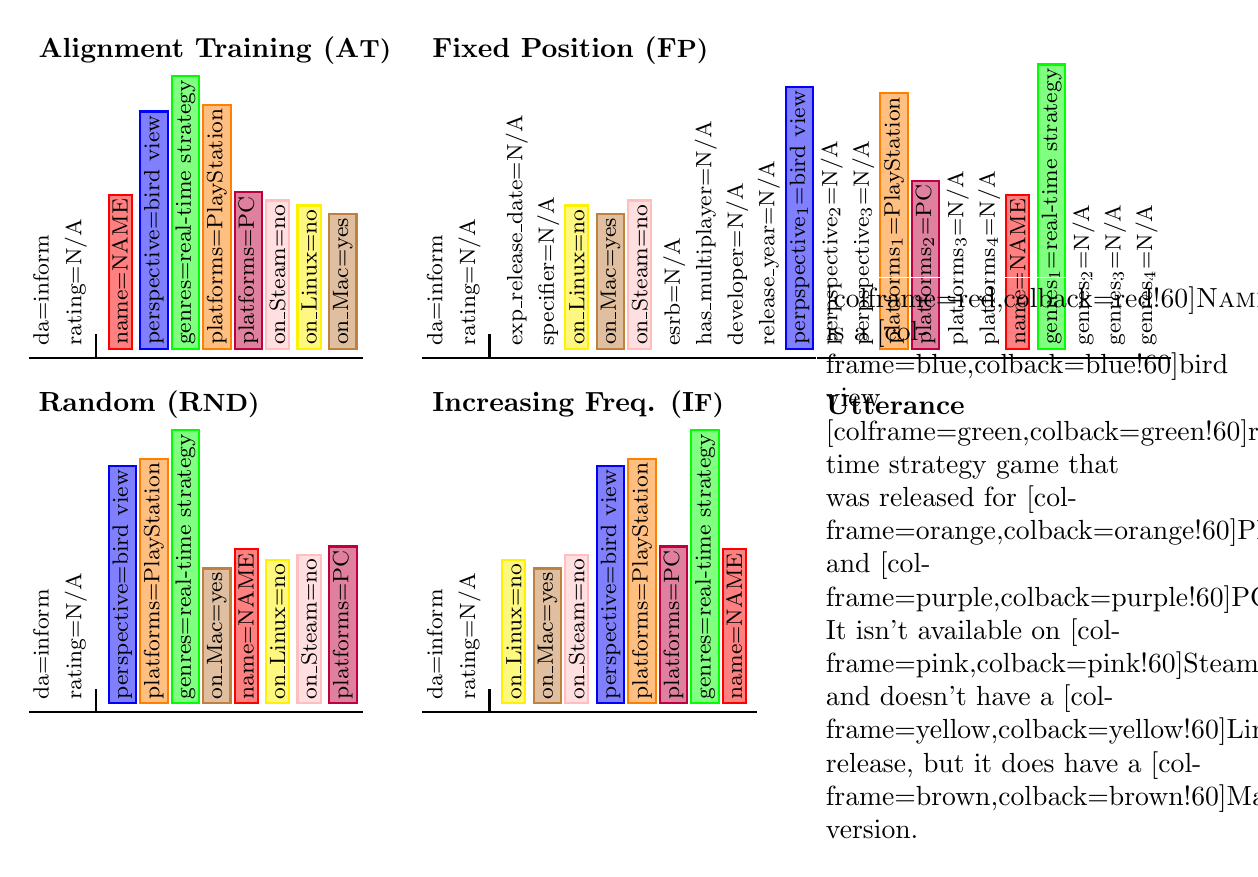
\begin{tikzpicture}[]


    \node[anchor=west] at (5.0,5.8) 
        {\textbf{Fixed Position \textsc{(F\small{P})}}};
    \node[anchor=west] at (0.0,5.8) 
        {\textbf{Alignment Training \textsc{(A\small{T})}}};
    \draw[thick] (0.85,1.9) -- (0.85,2.2);
    \draw[thick] (0,1.9) -- (4.25,1.9);
    \draw[thick] (5 + 0.85,1.9) -- (5 + 0.85,2.2);
    \draw[thick] (5 + 0,1.9) -- (10.25+ 4.25,1.9);
    \draw[thick] (0.85,-2.6) -- (0.85,-2.3);
    \draw[thick] (0,-2.6) -- (4.25,-2.6);
    \draw[thick] (5+0.85,-2.6) -- (5+0.85,-2.3);
    \draw[thick] (5+0,-2.6) -- (5+4.25,-2.6);

    \node[anchor=north west,inner sep=0.5mm,rotate=90] at (0,2) 
        {\footnotesize da=inform};
    \node[anchor=north west,inner sep=0.5mm,rotate=90] at (0.4,2) 
        {\footnotesize rating=N/A};
    \node[anchor=north west,rotate=90,inner sep=0.5mm,draw=red,thick,fill=red!50] 
        at (0.2 + 0.8,2) 
        {\footnotesize name=NAME};
    \node[anchor=north west,rotate=90,inner sep=0.5mm,draw=blue,thick,fill=blue!50] 
        at (0.2 + 1.2,2) {\footnotesize perspective=bird view};
    \node[anchor=north west,rotate=90,inner sep=0.5mm,draw=green,thick,
          fill=green!50] 
        at (0.2 + 1.6,2) {\footnotesize genres=real-time strategy};
    \node[anchor=north west,rotate=90,inner sep=0.5mm,draw=orange,thick,
          fill=orange!50] 
        at (0.2 + 2.0,2) {\footnotesize platforms=PlayStation};
    \node[anchor=north west,rotate=90,inner sep=0.5mm,draw=purple,thick,
          fill=purple!50] 
        at (0.2 + 2.4,2) {\footnotesize platforms=PC};
    \node[anchor=north west,rotate=90,inner sep=0.5mm,draw=pink,thick,
          fill=pink!50] 
        at (0.2 + 2.8,2) {\footnotesize on\_Steam=no};
    \node[anchor=north west,rotate=90,inner sep=0.5mm,draw=yellow,thick,
          fill=yellow!50] 
        at (0.2 + 3.2,2) {\footnotesize on\_Linux=no};
    \node[anchor=north west,rotate=90,inner sep=0.5mm,draw=brown,thick,
          fill=brown!50] 
        at (0.2 + 3.6,2) {\footnotesize on\_Mac=yes};


\node[anchor=north west,inner sep=0.5mm,rotate=90] at (5 + 0,2) 
    {\footnotesize da=inform};
\node[anchor=north west,inner sep=0.5mm,rotate=90] at (5 + 0.4,2) 
    {\footnotesize rating=N/A};
\node[anchor=north west,rotate=90,inner sep=0.5mm] 
    at (5.2 + 0.8,2) 
    {\footnotesize exp\_release\_date=N/A};
\node[anchor=north west,rotate=90,inner sep=0.5mm] 
    at (5.2 + 1.2,2) 
    {\footnotesize specifier=N/A};
\node[anchor=north west,rotate=90,inner sep=0.5mm,draw=yellow,thick,fill=yellow!50] 
    at (5.2 + 1.6,2) 
    {\footnotesize on\_Linux=no};
\node[anchor=north west,rotate=90,inner sep=0.5mm,draw=brown,thick,fill=brown!50] 
    at (5.2 + 2.0,2) 
    {\footnotesize on\_Mac=yes};
\node[anchor=north west,rotate=90,inner sep=0.5mm,draw=pink,thick,fill=pink!50] 
    at (5.2 + 2.4,2) 
    {\footnotesize on\_Steam=no};
\node[anchor=north west,rotate=90,inner sep=0.5mm] 
    at (5.2 + 2.8,2) 
    {\footnotesize esrb=N/A};
\node[anchor=north west,rotate=90,inner sep=0.5mm] 
    at (5.2 + 3.2,2) 
    {\footnotesize has\_multiplayer=N/A};

   % ['inform', 'rating=N/A', 'exp_release_date=N/A', 'specifier=N/A', 'has_linux_release=no', 'has_mac_release=yes', 'available_on_steam=no', 'esrb=N/A', 'has_multiplayer=N/A', 'developer=N/A', 'release_year=N/A', 'player_perspective=bird view', 'player_perspective=N/A', 'player_perspective=N/A', 'platforms=PlayStation', 'platforms=PC', 'platforms=N/A', 'platforms=N/A', 'name=PLACEHOLDER', 'genres=real-time strategy', 'genres=N/A', 'genres=N/A', 'genres=N/A']
\node[anchor=north west,rotate=90,inner sep=0.5mm] 
    at (5.2 + 3.6,2) 
    {\footnotesize developer=N/A};
\node[anchor=north west,rotate=90,inner sep=0.5mm] 
    at (5.2 + 4.0,2) 
    {\footnotesize release\_year=N/A};
\node[anchor=north west,rotate=90,inner sep=0.5mm,draw=blue,thick,fill=blue!50] 
    at (5.2 + 4.4,2) 
    {\footnotesize perpspective\textsubscript{1}=bird view};
\node[anchor=north west,rotate=90,inner sep=0.5mm] 
    at (5.2 + 4.8,2) 
    {\footnotesize perpspective\textsubscript{2}=N/A};
\node[anchor=north west,rotate=90,inner sep=0.5mm] 
    at (5.2 + 5.2,2) 
    {\footnotesize perpspective\textsubscript{3}=N/A};
\node[anchor=north west,rotate=90,inner sep=0.5mm,draw=orange,thick,fill=orange!50] 
    at (5.2 + 5.6,2) 
    {\footnotesize platforms\textsubscript{1}=PlayStation};
\node[anchor=north west,rotate=90,inner sep=0.5mm,draw=purple,thick,fill=purple!50] 
    at (5.2 + 6.0,2) 
    {\footnotesize platforms\textsubscript{2}=PC};
\node[anchor=north west,rotate=90,inner sep=0.5mm] 
    at (5.2 + 6.4,2) 
    {\footnotesize platforms\textsubscript{3}=N/A};
\node[anchor=north west,rotate=90,inner sep=0.5mm] 
    at (5.2 + 6.8,2) 
    {\footnotesize platforms\textsubscript{4}=N/A};
\node[anchor=north west,rotate=90,inner sep=0.5mm,draw=red,thick,fill=red!50] 
    at (5.2 + 7.2,2) 
    {\footnotesize name=NAME};
\node[anchor=north west,rotate=90,inner sep=0.5mm,draw=green,thick,fill=green!50] 
    at (5.2 + 7.6,2) 
    {\footnotesize genres\textsubscript{1}=real-time strategy};
\node[anchor=north west,rotate=90,inner sep=0.5mm] 
    at (5.2 + 8.0,2) 
    {\footnotesize genres\textsubscript{2}=N/A};
\node[anchor=north west,rotate=90,inner sep=0.5mm] 
    at (5.2 + 8.4,2) 
    {\footnotesize genres\textsubscript{3}=N/A};
\node[anchor=north west,rotate=90,inner sep=0.5mm] 
    at (5.2 + 8.8,2) 
    {\footnotesize genres\textsubscript{4}=N/A};


%\node[anchor=north west,rotate=90] at (1.5,2) {genres=platformer};
%\node[anchor=north west,rotate=90] at (2,2) {genres=puzzle};
%\node[anchor=north west,rotate=90] at (2.5,2) {perspective=side vew};
%\node[anchor=north west,rotate=90] at (3,2) {name=NAME};
%\node[anchor=north west,rotate=90] at (3.5,2) {name=NAME};
%\node[anchor=north west,rotate=90] at (4,2) {name=NAME};
%\node[anchor=north west,rotate=90] at (4.5,2) {name=NAME};
%
%
%\node[anchor=north west,rotate=90] at (5.5+0,2) {\small give opinion};
%\node[anchor=north west,rotate=90] at (5.5+0.5,2) {\small rating=good};
%\node[anchor=north west,rotate=90] at (5.5+1,2) {\small genres=adventure};
%\node[anchor=north west,rotate=90] at (5.5+1.5,2) {genres=platformer};
%\node[anchor=north west,rotate=90] at (5.5+2,2) {genres=puzzle};
%\node[anchor=north west,rotate=90] at (5.5+2.5,2) {perspective=side vew};
%\node[anchor=north west,rotate=90] at (5.5+3,2) {name=NAME};
%\node[anchor=north west,rotate=90] at (5.5+3.5,2) {name=NAME};
%\node[anchor=north west,rotate=90] at (5.5+4,2) {name=NAME};
%\node[anchor=north west,rotate=90] at (10+0,2) {give opinion};
%\node[anchor=north west,rotate=90] at (10+0.5,2) {rating=good};
%\node[anchor=north west,rotate=90] at (10+1,2) {genres=adventure};
%\node[anchor=north west,rotate=90] at (10+1.5,2) {genres=platformer};
%\node[anchor=north west,rotate=90] at (10+2,2) {genres=puzzle};
%\node[anchor=north west,rotate=90] at (10+2.5,2) {perspective=side vew};
%\node[anchor=north west,rotate=90] at (10+3,2) {name=NAME};
%\node[anchor=north west,rotate=90] at (10+3.5,2) {name=NAME};
%\node[anchor=north west,rotate=90] at (10+4,2) {name=NAME};
%\node[anchor=north west,rotate=90] at (10+4.5,2) {name=NAME};
%
%



%['give_opinion', 'rating=good', 'genres=adventure', 'genres=platformer', 'genres=puzzle', 'player_perspective=side view', 'name=PLACEHOLDER']


%#
%#

%['inform', 'rating=N/A', 'exp_release_date=N/A', 'specifier=N/A', 'has_linux_release=no', 'has_mac_release=yes', 'available_on_steam=no', 'esrb=N/A', 'has_multiplayer=N/A', 'developer=N/A', 'release_year=N/A', 'player_perspective=bird view', 'player_perspective=N/A', 'player_perspective=N/A', 'platforms=PlayStation', 'platforms=PC', 'platforms=N/A', 'platforms=N/A', 'name=PLACEHOLDER', 'genres=real-time strategy', 'genres=N/A', 'genres=N/A', 'genres=N/A']


%inc_freq_delex
%['inform', 'rating=N/A', 'has_linux_release=no', 'has_mac_release=yes', 'available_on_steam=no', 'player_perspective=bird view', 'platforms=PlayStation', 'platforms=PC', 'name=PLACEHOLDER', 'genres=real-time strategy']

\node[anchor=north west,inner sep=0.5mm,rotate=90] at (0,-2.5) 
    {\footnotesize da=inform};
\node[anchor=north west,inner sep=0.5mm,rotate=90] at (0.4,-2.5) 
    {\footnotesize rating=N/A};
\node[anchor=north west,rotate=90,inner sep=0.5mm,draw=blue,thick,fill=blue!50] 
    at (0.2 + 0.8,-2.5) 
    {\footnotesize perspective=bird view};

\node[anchor=north west,rotate=90,inner sep=0.5mm,draw=orange,thick,fill=orange!50] 
    at (0.2 + 1.2,-2.5) 
    {\footnotesize platforms=PlayStation};
\node[anchor=north west,rotate=90,inner sep=0.5mm,draw=green,thick,fill=green!50] 
    at (0.2 + 1.6,-2.5) 
    {\footnotesize genres=real-time strategy};


\node[anchor=north west,rotate=90,inner sep=0.5mm,draw=brown,thick,fill=brown!50] 
    at (0.2 + 2.0,-2.5) 
    {\footnotesize on\_Mac=yes};
\node[anchor=north west,rotate=90,inner sep=0.5mm,draw=red,thick,fill=red!50] 
    at (0.2 + 2.4,-2.5) 
    {\footnotesize name=NAME};

\node[anchor=north west,rotate=90,inner sep=0.5mm,draw=yellow,thick,fill=yellow!50] 
    at (0.2 + 2.8,-2.5) 
    {\footnotesize on\_Linux=no};
\node[anchor=north west,rotate=90,inner sep=0.5mm,draw=pink,thick,fill=pink!50] 
    at (0.2 + 3.2,-2.5) 
    {\footnotesize on\_Steam=no};
\node[anchor=north west,rotate=90,inner sep=0.5mm,draw=purple,thick,fill=purple!50] 
    at (0.2 + 3.6,-2.5) 
    {\footnotesize platforms=PC};

    \node[anchor=west] at (0,1.3) {\textbf{Random \textsc{(R\small{ND})}}};



\node[anchor=north west,inner sep=0.5mm,rotate=90] at (5 + 0,-2.5) 
    {\footnotesize da=inform};
\node[anchor=north west,inner sep=0.5mm,rotate=90] at (5 + 0.4,-2.5) 
    {\footnotesize rating=N/A};
\node[anchor=north west,rotate=90,inner sep=0.5mm,draw=yellow,thick,fill=yellow!50] 
    at (5.2 + 0.8,-2.5) 
    {\footnotesize on\_Linux=no};
\node[anchor=north west,rotate=90,inner sep=0.5mm,draw=brown,thick,fill=brown!50] 
    at (5.2 + 1.2,-2.5) 
    {\footnotesize on\_Mac=yes};
\node[anchor=north west,rotate=90,inner sep=0.5mm,draw=pink,thick,fill=pink!50] 
    at (5.2 + 1.6,-2.5) 
    {\footnotesize on\_Steam=no};

\node[anchor=north west,rotate=90,inner sep=0.5mm,draw=blue,thick,fill=blue!50]
    at (5.2 + 2.0,-2.5) 
    {\footnotesize perspective=bird view};
\node[anchor=north west,rotate=90,inner sep=0.5mm,draw=orange,thick,fill=orange!50] 
    at (5.2 + 2.4,-2.5) 
    {\footnotesize platforms=PlayStation};
\node[anchor=north west,rotate=90,inner sep=0.5mm,draw=purple,thick,fill=purple!50] 
    at (5.2 + 2.8,-2.5) 
    {\footnotesize platforms=PC};

\node[anchor=north west,rotate=90,inner sep=0.5mm,draw=green,thick,fill=green!50] 
    at (5.2 + 3.2,-2.5) 
    {\footnotesize genres=real-time strategy};
\node[anchor=north west,rotate=90,inner sep=0.5mm,draw=red,thick,fill=red!50] 
    at (5.2 + 3.6,-2.5) 
    {\footnotesize name=NAME};
%has_linux_release=no', 'has_mac_release=yes', 'available_on_steam=no', 'player_perspective=bird view', 'platforms=PlayStation', 'platforms=PC', 'name=PLACEHOLDER', 'genres=real-time strategy'
    \node[anchor=west] at (5.0,1.3) {\textbf{Increasing Freq. \textsc{(I\small{F})}}};


%\node[anchor=north west,inner sep=0.5mm,rotate=90] at (10 + 0,-2.5) 
%    {\footnotesize da=inform};
%\node[anchor=north west,inner sep=0.5mm,rotate=90] at (10 + 0.4,-2.5) 
%    {\footnotesize rating=N/A};
%
%\node[anchor=north west,rotate=90,inner sep=0.5mm,draw=red,thick,fill=red!50] 
%    at (10.2 + 0.8,-2.5) 
%    {\footnotesize name=NAME};
%
%\node[anchor=north west,rotate=90,inner sep=0.5mm,draw=green,thick,fill=green!50] 
%    at (10.2 + 1.2,-2.5) 
%    {\footnotesize genres=real-time strategy};
%
%    \node[anchor=north west,rotate=90,inner sep=0.5mm,draw=purple,thick,fill=purple!50] 
%    at (10.2 + 1.6,-2.5) 
%    {\footnotesize platforms=PC};
%\node[anchor=north west,rotate=90,inner sep=0.5mm,draw=orange,thick,fill=orange!50] 
%    at (10.2 + 2.0,-2.5) 
%    {\footnotesize platforms=PlayStation};
%
%\node[anchor=north west,rotate=90,inner sep=0.5mm,draw=blue,thick,fill=blue!50]
%    at (10.2 + 2.4,-2.5) 
%    {\footnotesize perspective=bird view};
%\node[anchor=north west,rotate=90,inner sep=0.5mm,draw=pink,thick,fill=pink!50] 
%    at (10.2 + 2.8,-2.5) 
%    {\footnotesize on\_Steam=no};
%\node[anchor=north west,rotate=90,inner sep=0.5mm,draw=brown,thick,fill=brown!50] 
%    at (10.2 + 3.2,-2.5) 
%    {\footnotesize on\_Mac=yes};
%\node[anchor=north west,rotate=90,inner sep=0.5mm,draw=yellow,thick,fill=yellow!50] 
%    at (10.2 + 3.6,-2.5) 
%    {\footnotesize on\_Linux=no};
%




%has_linux_release=no', 'has_mac_release=yes', 'available_on_steam=no', 'player_perspective=bird view', 'platforms=PlayStation', 'platforms=PC', 'name=PLACEHOLDER', 'genres=real-time strategy'
%    \node[anchor=west] at (10.0,1.3) {\textbf{Decreasing Freq.}};




    \node[anchor=west] at (10, 1.3) {\textbf{Utterance}};
\node[text width=5.0cm,draw=white,anchor=west] at (10,-0.7) {
    {\mybox[colframe=red,colback=red!60]{\textsc{Name}}} is a 
    \mybox[colframe=blue,colback=blue!60]{bird view} 
    \mybox[colframe=green,colback=green!60]{real-time strategy} 
    game that was released for 
    \mybox[colframe=orange,colback=orange!60]{PlayStation} and 
    \mybox[colframe=purple,colback=purple!60]{PC.} It isn't available on 
    \mybox[colframe=pink,colback=pink!60]{Steam} and doesn't have a 
    \mybox[colframe=yellow,colback=yellow!60]{Linux} release, but it does have
    a \mybox[colframe=brown,colback=brown!60]{Mac} version.
};


\end{tikzpicture}

\caption{Example MR linearization strategies for the utterance above from the
    ViGGO training set.}
\label{fig:linstrats}
\end{figure*}


\paragraph{Random (\textsc{Rnd})} In the \lsname{random} linearization
(\lsshort{Rnd}), we randomly order the attribute-value pairs for a given MR.
This strategy serves as a baseline for determining if linearization 
matters at all for faithfulness. \lsshort{Rnd} is similar to token level noise
used in denoising auto-encoders \cite{wang2019} and might
even improve faithfulness.  During training, we resample the ordering for each
example at every epoch.  We do not resample the validation set in order to
obtain stable results for model selection.

\paragraph{Increasing Frequency (\textsc{If})} In the \lsname{increasing
frequency} linearization (\lsshort{If}), we order the attribute-value pairs by
increasing frequency of occurrence in the training data (i.e., $\acount(\attr_i)
\le \acount(\attr_{i+1})$).  We hypothesize that placing frequently occurring
items in a consistent location may make it easier for $\model$ to realize
those items correctly, possibly at the expense of rarer items.

\paragraph{Fixed Position (\textsc{Fp})} We take  consistency one step further
and create a fixed ordering of all attributes, \textit{n.b.} not
attribute-values, ordering them in increasing frequency of occurrence on the
training set (i.e. every instance has the same order of attributes in the
encoder input). In this \lsname{fixed position} linearization (\lsshort{Fp}),
attributes that are not present in an MR are explicitly represented with an
\Val{N/A} value.  For list-valued slots, we determine the maximum length
list in the training data and create that many repeated slots in the input
sequence.  This linearization is feasible for datasets with a modest number of
unique attributes %(in our case Viggo has 14 attributes and E2E eight) 
but may 
not easily scale to 10s, 100s, or larger attribute vocabularies. 

\paragraph{Alignment Training (\textsc{At})} 

In the \lsname{alignment training} linearization (\lsshort{At}), during
training, the order of attribute-value pairs $\attr_1, \attr_2, \ldots,
\attr_\size{\mr}$ matches the order in which they are realized in the
corresponding training utterance.  This is feasible because in the majority of
cases, there is a one-to-one mapping of attribute-values and utterance
subspans.

%%  %Training $\model$ with this strategy yields a model
%%  %that is highly controllable, i.e. when conditioning on $\lin(\mr) = [\da, \attr_i, \attr_{i+1}, \ldots]$, $\model(\cdot|\lin(\mr);\theta)$ will 
%%  %place higher probability on utterances where $\attr_i$ is realized first,
%%  %followed by $\attr_{i+1}$, and so on.

We obtain this ordering using a manually constructed set of matching rules to
identify which utterance subspans correspond to each attribute-value pair
(see \autoref{sec:align}).

Crucially, \lsshort{At}~stands in contrast to the  first three strategies
(\lsshort{Rnd}, \lsshort{If}, and \lsshort{Fp}) which do not have any
correspondence between the the order of attribute-value pairs in $\lin(\mr)$
and the order in which they are realized in the corresponding utterance
$\utt$. %and as a  result, models trained with those strategies %are not controllable. 
%KM - Again, isn't this something you will show through your experiments?




At test time, when there is no reference utterance \lsshort{At}
cannot specify a linearization. However, models trained with \lsshort{At}
can generate an  utterance from an arbitrary utterance plan
$\attr_1, \attr_2, \ldots, \attr_{\size{\mr}}$ 
provided by an external source, such as an utterance planner model or human 
reference. {\color{red}See \autoref{fig:ctrlouts} for an example how an \lsshort{At}-trained model might follow three different plans for the same MR.}
%%  %. We refer to such an ordering as an {\em utterance plan}.
%%  %KM - I put in italics. This sentence implies it's the first time mentioned, but you mention t in the intro. Perhaps you can define it there? 

\begin{figure}
    \resizebox{.48\textwidth}{!}{%
        \begin{tabular}{l}
            \toprule
            $\lin\left(\mr\right) = \left[\textrm{inform}, 
                \textrm{name=Aromi}, \textrm{eat\_type=coffee shop}, 
                \textrm{area=city centre} \right]$\\
            $\hat{\utt} = \textit{Aromi is a coffee shop in the city 
                centre.}$\\
            \midrule
            $\lin\left(\mr\right) = \left[\textrm{inform}, 
                \textrm{eat\_type=coffee shop}, \textrm{name=Aromi}, 
                \textrm{area=city centre} \right]$\\
            $\hat{\utt} = \textit{There is a coffee shop called Aromi in the 
                city centre.}$\\
            \midrule
            $\lin\left(\mr\right) = \left[\textrm{inform}, 
                \textrm{eat\_type=coffee shop}, \textrm{area=city centre}, 
                \textrm{name=Aromi} \right]$\\
            $\hat{\utt} = \textit{For coffee in the centre of the city, try 
                Aromi.}$\\
            \bottomrule
        \end{tabular}
    }
    \caption{Example outputs ($\hat{\utt}$) from a controllable model, 
i.e. a S2S model trained with \lsshort{At} linearization, 
under different input utterance plans ($\lin\left(\mr\right)$).}
\label{fig:ctrlouts}
\end{figure}

